\documentclass[border=5pt]{standalone}
\usepackage{tikz}
\usepackage{amsmath}
\usetikzlibrary{arrows.meta}
\begin{document}
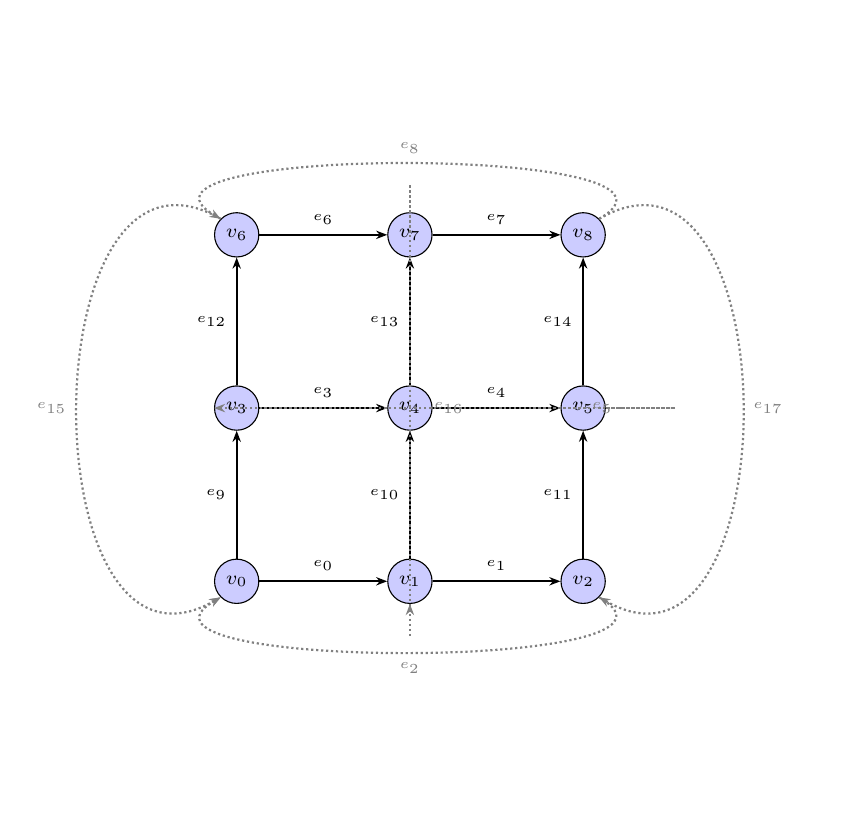
\begin{tikzpicture}[
  vertex/.style={circle, draw, fill=blue!20, minimum size=16pt, inner sep=0pt, font=\scriptsize},
  wrap/.style={->, thick, densely dotted, gray},
  >={Stealth[length=4pt]},
  scale=1.0
]
  % Grid spacing
  \def\s{2.2}

  % Vertices: row-major v0..v8
  \foreach \r in {0,1,2} {
    \foreach \c in {0,1,2} {
      \pgfmathtruncatemacro{\idx}{\r*3+\c}
      \node[vertex] (v\idx) at (\c*\s, \r*\s) {$v_{\idx}$};
    }
  }

  % Horizontal edges (reference: right)
  % Row 0: e0(v0->v1), e1(v1->v2), e2(v2->v0 wrap)
  \draw[->, thick] (v0) -- node[font=\tiny, above] {$e_0$} (v1);
  \draw[->, thick] (v1) -- node[font=\tiny, above] {$e_1$} (v2);
  % Row 1: e3(v3->v4), e4(v4->v5), e5(v5->v3 wrap)
  \draw[->, thick] (v3) -- node[font=\tiny, above] {$e_3$} (v4);
  \draw[->, thick] (v4) -- node[font=\tiny, above] {$e_4$} (v5);
  % Row 2: e6(v6->v7), e7(v7->v8), e8(v8->v6 wrap)
  \draw[->, thick] (v6) -- node[font=\tiny, above] {$e_6$} (v7);
  \draw[->, thick] (v7) -- node[font=\tiny, above] {$e_7$} (v8);

  % Vertical edges (reference: up)
  % Col 0: e9(v0->v3), e12(v3->v6), e15(v6->v0 wrap)
  \draw[->, thick] (v0) -- node[font=\tiny, left] {$e_9$} (v3);
  \draw[->, thick] (v3) -- node[font=\tiny, left] {$e_{12}$} (v6);
  % Col 1: e10(v1->v4), e13(v4->v7), e16(v7->v1 wrap)
  \draw[->, thick] (v1) -- node[font=\tiny, left] {$e_{10}$} (v4);
  \draw[->, thick] (v4) -- node[font=\tiny, left] {$e_{13}$} (v7);
  % Col 2: e11(v2->v5), e14(v5->v8), e17(v8->v2 wrap)
  \draw[->, thick] (v2) -- node[font=\tiny, left] {$e_{11}$} (v5);
  \draw[->, thick] (v5) -- node[font=\tiny, left] {$e_{14}$} (v8);

  % Wrap-around horizontal edges (dotted, curving outside the grid)
  % e2: v2 -> v0 (right wraps to left, row 0)
  \draw[wrap] (v2.south east) to[out=-30, in=-150]
    node[font=\tiny, below] {$e_2$} (v0.south west);
  % e5: v5 -> v3 (row 1)
  \draw[wrap] (v5.east) to[out=0, in=0, looseness=1.5]
    node[font=\tiny, right] {$e_5$} (v3.west);
  % e8: v8 -> v6 (row 2)
  \draw[wrap] (v8.north east) to[out=30, in=150]
    node[font=\tiny, above] {$e_8$} (v6.north west);

  % Wrap-around vertical edges (dotted, curving outside the grid)
  % e15: v6 -> v0 (top wraps to bottom, col 0)
  \draw[wrap] (v6.north west) to[out=150, in=-150, looseness=1.5]
    node[font=\tiny, left] {$e_{15}$} (v0.south west);
  % e16: v7 -> v1 (col 1)
  \draw[wrap] (v7.north) to[out=90, in=-90, looseness=1.2]
    node[font=\tiny, right, xshift=5pt] {$e_{16}$} (v1.south);
  % e17: v8 -> v2 (col 2)
  \draw[wrap] (v8.north east) to[out=30, in=-30, looseness=1.5]
    node[font=\tiny, right] {$e_{17}$} (v2.south east);

\end{tikzpicture}
\end{document}
